\chapter{ПРОГРАМНИЙ МОДУЛЬ ВИЗНАЧЕННЯ МЕТРИК ЦІЛЬОВОЇ ПРОГРАМИ ДЛЯ ПІДВИЩЕННЯ ЕФЕКТИВНОСТІ ДОСЛІДЖЕННЯ ЇЇ ПОТЕНЦІЙНО-НЕБЕЗПЕЧНИХ ДЕФЕКТІВ}
\label{3section::doc}\label{3section:id1}

\section{Структурна схема алгоритму та основні функціональні елементи}
\label{3section:id2}
Підчас аналізу предметної області мною була запропонована структурна схема програмно-технічного комплексу дослідження цільових програм на переповнення буфера 
\begin{figure} [h]
    \centering
    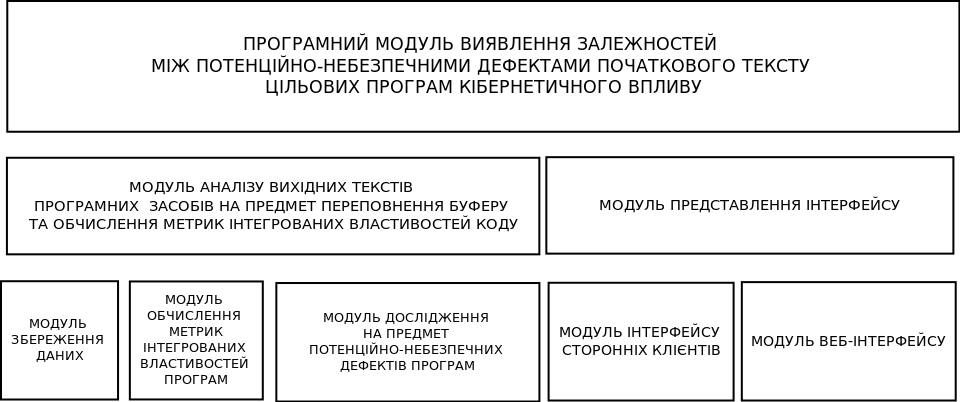
\includegraphics[width=16cm]{general_structure.png}
    \caption{Структурна схема модулю визначення метрик цільової програми}
    \label{fig:general_structure}
\end{figure}
(Рис \,\ref{fig:general_structure})

\section{Інтерфейс користувача}
\label{3section:id3}

\section{Керівництво щодо розгортання та експлуатації}
\label{3section:id4}

\section*{Висновки}
\addcontentsline{toc}{section}{Висновки}
Отже,
